%!TEX root = main_arduino_intro.tex

\chapter{Display}

In order to display the temperature of our sample cooling setup, we will connect a display to our Arduino. Displays come in many different shapes and forms, form the monitor you might be reading this on to simple \ac{led} seven-segmant displays. An overview of various displays that are ready to be deployed on Arduino can, e.g., be found \href{https://www.arduino.cc/reference//en/libraries/category/display/}{here}. For our specific case, a simple seven-segment display will do the trick to display the temperature.

\subsection{Seven-segment displays} 

\begin{figure}[htb]
    \centering
    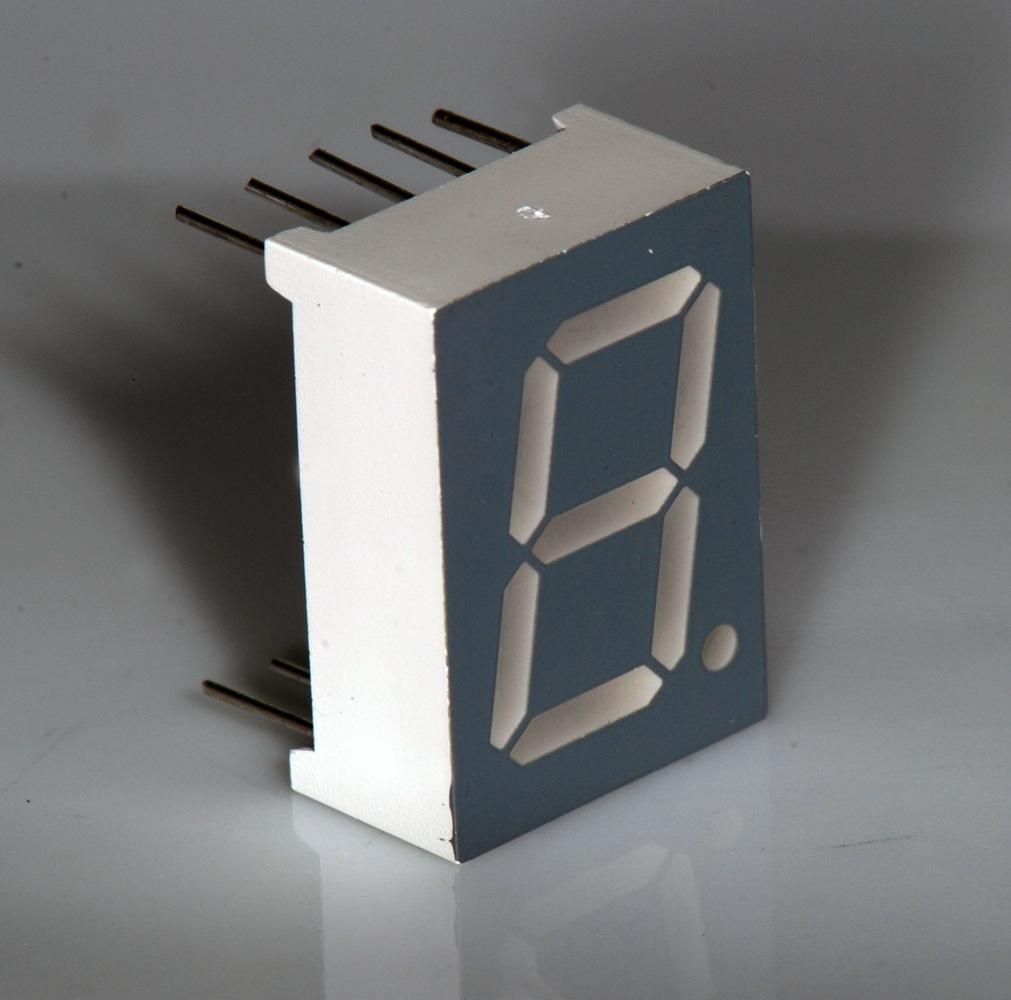
\includegraphics[height=4cm]{graphics/02_display/7seg_photo.jpg} \hspace{1.5cm}
    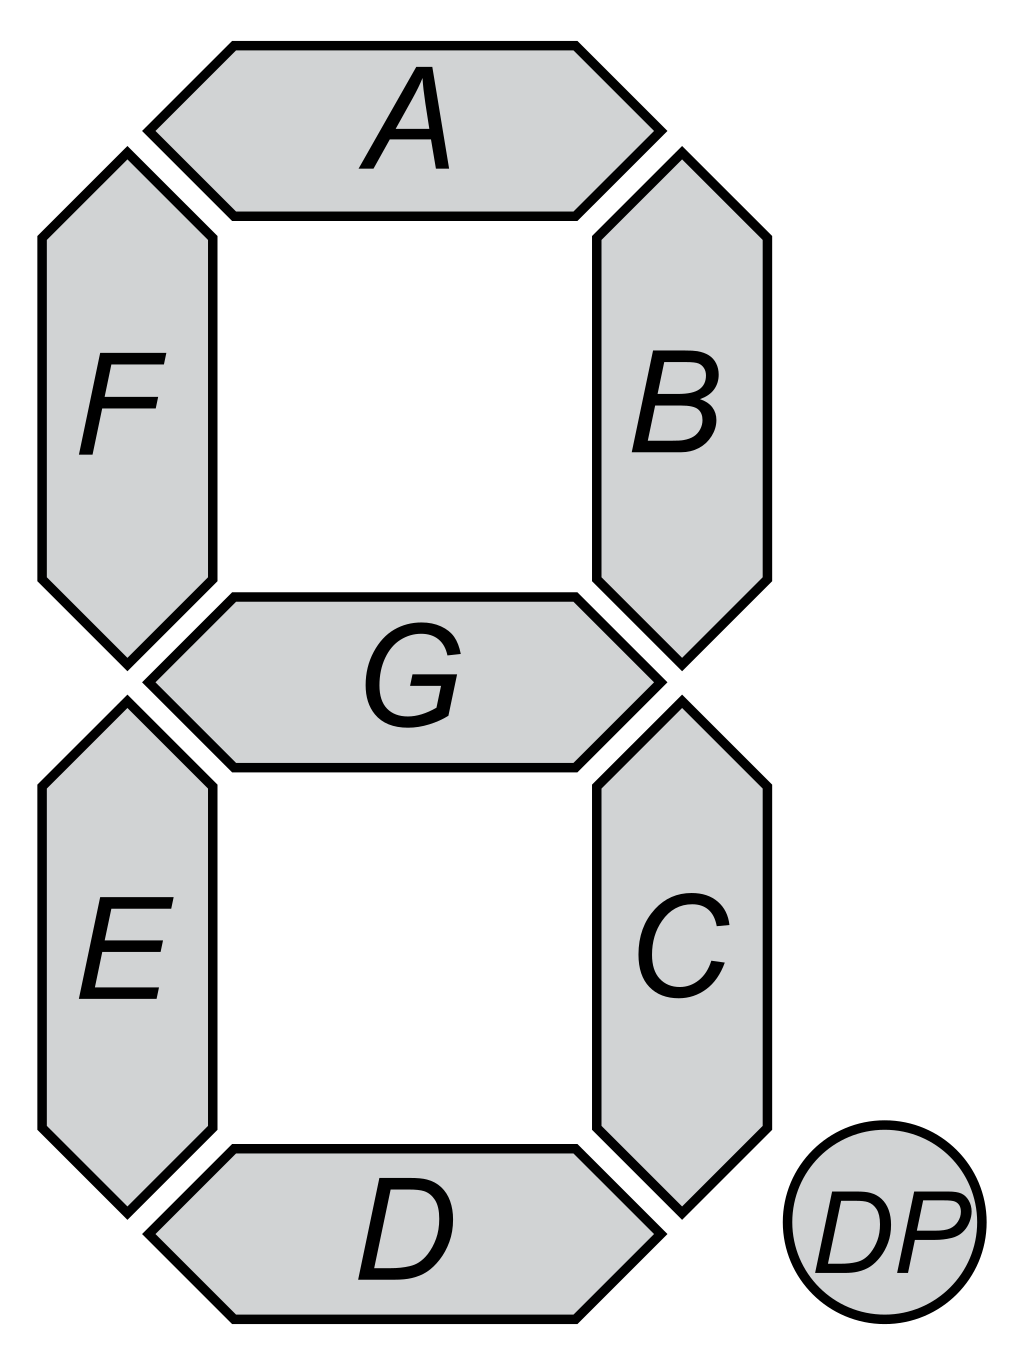
\includegraphics[height=4cm]{graphics/02_display/7seg_schematic.png}
    \caption{Seven-segment display: photo (left) and schematic (right). Credit: \href{https://en.wikipedia.org/wiki/Seven-segment_display\#/media/File:Seven_segment_01_Pengo.jpg}{Peter Halasz (left)} and \href{https://en.wikipedia.org/wiki/Seven-segment_display\#/media/File:7_Segment_Display_with_Labeled_Segments.svg}{Uln2003 (right)} via Wikipedia. License: \href{https://creativecommons.org/licenses/by-sa/3.0/}{CC by SA-3.0 (left)}, \href{https://en.wikipedia.org/wiki/Seven-segment_display\#/media/File:7_Segment_Display_with_Labeled_Segments.svg}{Public domain -- CC0 (right)}}
    \label{fig:display:7seg}
\end{figure}
As displayed in Figure~\ref{fig:display:7seg}, seven-segment displays contain seven individual segments that allow us to display any nummer and even some letters. In addition, they can contain a decimal point. The right hand figure shows the schematic and typical labeling of a seven-segment display. Each segment is its own \ac{led} and we could drive these \acp{led} by using multiple \ac{io} pins. However, in order display multiple numbers, the number of \ac{io} pins that we would use up would very fast become too extensive. Figure~\ref{fig:display:7seg} shows that the seven-segment display has five pins on top and, not shown here, also five connectors on the bottom. For each seven-segment display you could look up the wiring diagram and notice that each segment has its own connection and that they have a total of two common grounds.

Chips such as 74HC595 that allow us to convert serial into parallel data allow us to effectively control multiple eight outputs, as required for such a display, with one only a few pins.
\begin{figure}[tb]
    \centering
    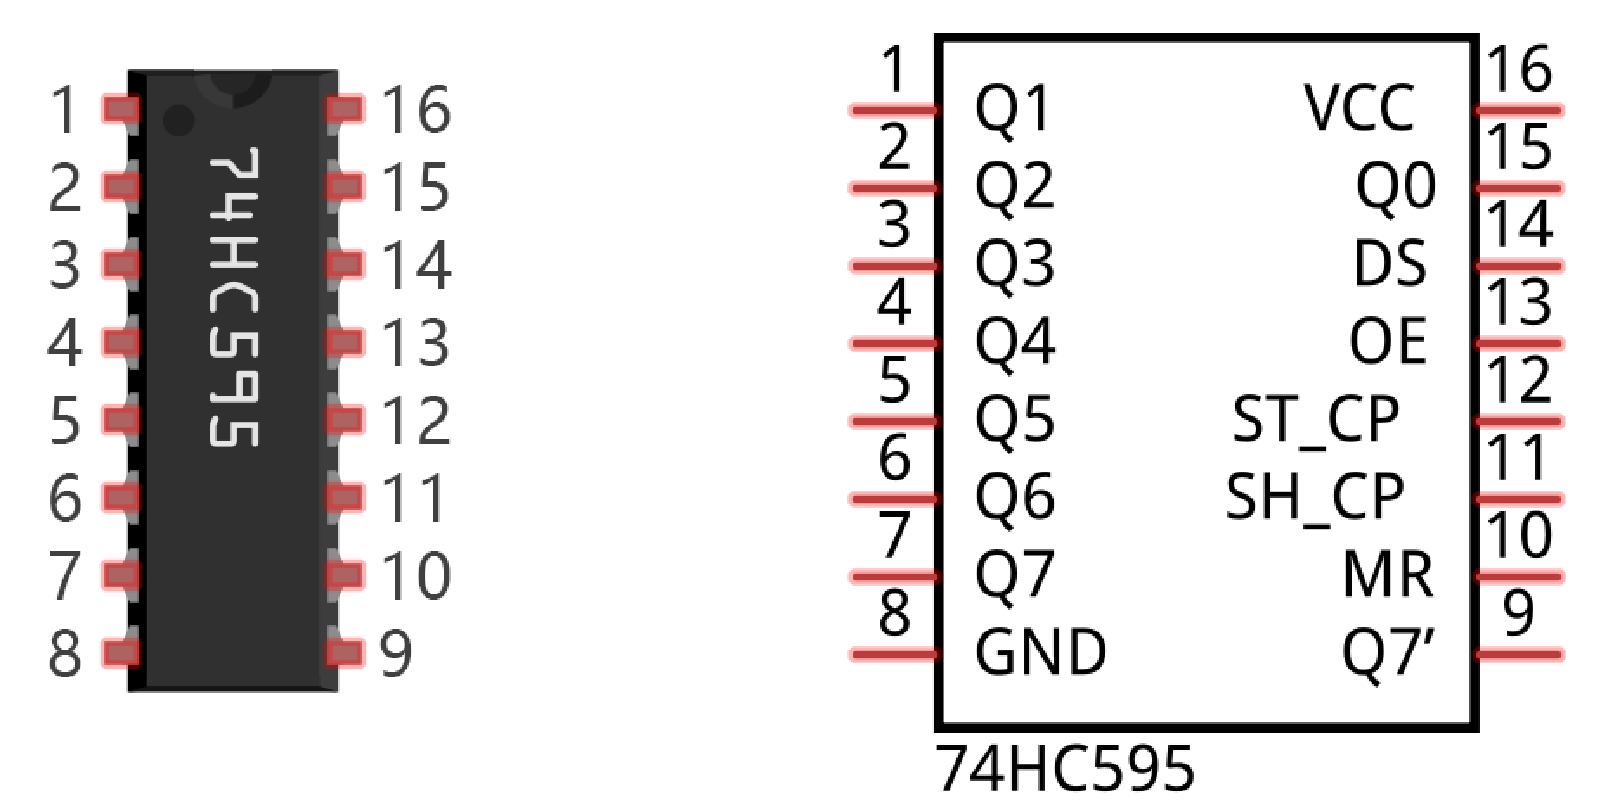
\includegraphics[]{graphics/02_display/74hc595.png}
    \caption{Schematic and pin names of a 74HC595 chip. Credit: \href{https://github.com/Freenove/Freenove_Ultimate_Starter_Kit_for_Raspberry_Pi}{Freenove}, License: \href{https://www.creativecommons.org/licenses/by-nc-sa/3.0/deed.en_US}{CC BY-NC-SA 3.0}}
    \label{fig:display:74hc595}
\end{figure}
Figure~\ref{fig:display:74hc595} shows a the schematic and pin names of such a chip. Note the notch on the top of the schematic that each chip contains in order to provide you with a reference on the pin assignments. You can in fact find various versions of this chip from different manufacturers, e.g., the datasheet for the Texas Instruments version can be found \href{https://www.ti.com/lit/ds/symlink/sn74hc595.pdf?ts=1636228778140&ref_url=https%253A%252F%252Fwww.google.com%252F}{here}. Generally, the pins have the following purposes:

\begin{center}
\begin{tabular}{lll}
    \hline
    \textbf{Pin name}   &   \textbf{Pin number} &   \textbf{Description}    \\
    \hline \hline
    Q0 - Q7             &   1-7, 15             &   Parallel data output \\
    GND                 &   8                   &   Ground \\
    Q7'                 &   9                   &   Serial data output \\
    MR                  &   10                  &   Remove shift register \\
    SH\_CP              &   11                  &   Serial shift clock \\
    ST\_CP              &   12                  &   Parallel update output \\
    OE                  &   13                  &   Enable output \\
    DS                  &   14                  &   Serial data input \\
    \hline
\end{tabular}
\end{center}

As indicated by the names, the parallel data output pins are the eight pins that can be connected to the individual \acp{led} of a seven-segment system. The GND pin provides the ground connection of the chip. The serial data output (Q7') can be used to connect another 74HC595 chip in series. The MR and SH\_CP take care of clearing the shift register and timing when a shift happens. The ST\_CT triggers an update in the parallel output and the OE pin enables this output. Finally, the DS pin is where the serial input is given. 

\morebox{Want do build your own seven segment display driver?}{Detailed instructions on how to use a 74HC595 chip to drive a seven segment display can be found online, e.g., on in chapter 17 of \href{https://github.com/Freenove/Freenove_Ultimate_Starter_Kit_for_Raspberry_Pi/blob/master/Tutorial.pdf}{this tutorial}. Building such a driver is outside the scope of our workshop, however, it might be useful for you to read and understand the shifting itself and how it works. Please have a look at the mentioned tutorial.}

\section{Adafruit four digit, seven-segment display with backpack}